%-----------------------------------------------------------------------
%
%\documentclass[referee]{aa} % for a referee version
%\documentclass[onecolumn]{aa} % for a paper on 1 column  
%\documentclass[longauth]{aa} % for the long lists of affiliations 
%\documentclass[letter]{aa} % for the letters 
%\documentclass[bibyear]{aa} % if the references are not structured 
%                              according to the author-year natbib style

%
\documentclass{aa}  

%
\usepackage{graphicx}
%%%%%%%%%%%%%%%%%%%%%%%%%%%%%%%%%%%%%%%%
\usepackage{txfonts}
%%%%%%%%%%%%%%%%%%%%%%%%%%%%%%%%%%%%%%%%
\usepackage{hyperref}
\hypersetup{colorlinks=true,allcolors=[rgb]{0,0,0.8}}
% SI units?
\usepackage{siunitx}
\usepackage{todonotes}
% To add links in your PDF file, use the package "hyperref"
% with options according to your LaTeX or PDFLaTeX drivers.
%
\usepackage{showyourwork}
\begin{document} 


   \title{Measuring the dust opacity of the debris disk around HD 107146 with transit photometry}

   %\subtitle{Subtitle}

   \author{A. Uthor1
          \inst{1}
          \and
          A. Uthor2\inst{2}\fnmsep\thanks{Just to show the usage
          of the elements in the author field}
          }

   \institute{Institute1, University1,
              Address1\\
              \email{e@mail1}
         \and
             Institute2, University2,
              Address2\\
             \email{e@mail2}
             \thanks{The university of heaven temporarily does not
                     accept e-mails}
             }

   \date{Received \today; accepted Month day, year}

% \abstract{}{}{}{}{} 
% 5 {} token are mandatory
 
  \abstract
  % context heading (optional)
  % {} leave it empty if necessary  
   {Differential photometry has been essential for probing galactic structure and composition. Using a background object the opacity of interstellar dust can be determined using the Beer-Lambert law. This method can also be used to probe dusty debris disks, with the added benefit of being able to use transiting background objects that have been imaged before being extincted by the disk. The relative motion of the HD 107146 disk and the Vermin galaxy has lead to the disk occulting the background galaxy starting in 2011. Three observation campaigns have imaged the occultation from 2004 until 2019.}
  % aims heading (mandatory)
   {We aim to use differential transit photometry to independently estimate the optical depth of dust in the HD 107146 debris disk using the Vermin galaxy as a background light source. }
  % methods heading (mandatory)
   {(Image processing/cleanup?) We use HST/STIS observations from 2011 to 2019 to build a surface brightness model of the disk. The model is then subtracted from the observations to remove the disk flux, which leaves only the extincted galaxy in the image. Then we select one 2011 epoch as the reference observation. Assuming that the optical depth is proportional to the surface brightness of the dust, we find the optical depth and its posterior by minimizing the residual sum of squares of the $\chi^2$ residuals of the extincted galaxies and reference as a function of the optical depth and other nuisance parameters using a MCMC method.}
  % results heading (mandatory)
   {We find an upper limit on the optical depth of $10^{-4}-10^{-3}$ for the dust in the HD 107146 disk. This new limit is close to the detection limit of our method. Importantly, we have not needed to a-priory estimate a constant mean dust density in the disk and find a mean dust density of $1.5 \pm 0.025 \mathrm{~g} \mathrm{~cm}^{-3}$ and opacity of $\approx 1.55 \times 10^{-18} \mathrm{~cm}^{2} / \mathrm{g} $ in the disk.}
  % conclusions heading (optional), leave it empty if necessary 
   {}

   \keywords{kw1 --
                kw2 --
                kw3
               }

   \maketitle
%
%-------------------------------------------------------------------

\section{Introduction}
\label{sec:introduction}

% \todo[inline]{Importance of dust}

% \todo[inline]{debris disk around stars}

% \todo[inline]{take out galaxies}

% \todo[inline]{introduce HD 107146}

% \todo[inline]{introduce obs/program}

% \todo[inline]{van Sluijs (idea and problems)}
% \todo[inline]{motivation for our method}

% \todo[inline]{orient on van Sluijs, introduce system, obs etc.}

The processes in debris disks are important for a significant part of the life of solar systems, specifically with regards to planet formation. Our understanding is based on observations, and increasingly on models of the physical processes themselves. These models rest on assumptions that are difficult to validate. Methods to probe disks, specifically at small particle sizes which give hints about the governing processes in discs such as collisional cascades, grain agglomeration and planetesimal formation are hence needed.

Previously, galactic astronomy was in a similar situation with regards to interstellar dust. It was widely assumed that (spiral) galaxies are semi-transparent to their own starlight, and thus must contain little dust. \cite{white1992direct} and later \cite{james1993measurement} for the first time used differential photometry to directly measure the optical depth of dust in occulting galaxy pairs. This method uses the extinction of background light through some foreground medium, e.g. interstellar dust, to find the optical depth of the medium according to the Beer-Lambert law, see \autoref{eq:beer_lamber_law}.
\begin{equation}
\label{eq:beer_lamber_law}
    T=\frac{\Phi_{\nu,1}}{\Phi_{\nu,0}}=e^{-\tau_{\nu}}
    % \frac{\mathrm{d} \Phi_{\nu}}{\mathrm{d} l}=-\tau_{\nu} \Phi_{\nu},
\end{equation}
where $T$ is the transmittance, $\Phi_{\nu,0}$, $\Phi_{\nu,1}$ is the flux at frequency $\nu$ before and after passing through the medium, respectively. $\tau_{\nu}$ is the optical depth of the medium which can be expressed in terms of the mediums density $\rho$, opacity $\kappa$, optical path length $l$ and surface density $\Sigma$ as shown in \autoref{eq:optical_depth}.
\begin{equation}
\label{eq:optical_depth}
    \tau_{v}=\int \rho \kappa_{v} d l=\kappa_{v} \Sigma
\end{equation}
The optical depth for an occulting, opaque and extended foreground $F$ and background $G$ source is then given by \autoref{eq:occ_pair}, where the second term separates the observations which is only possible if both models $F^{\prime}$ and $B^{\prime}$ are known. \citep{white2000seeing}
\begin{equation}
\label{eq:occ_pair}
    e^{-\tau^{\prime}}=\frac{\left\langle F+B e^{-\tau}\right\rangle-F^{\prime}}{B^{\prime}} \cong \frac{\left(F-F^{\prime}\right)}{B^{\prime}}+\frac{B}{B^{\prime}} e^{-\tau}
\end{equation}

When using this method for galactic astronomy one major disadvantage is that the relative motion of the two galaxies is often not sufficient to fully image the unocculted background galaxy. This means that the galaxies have to partially overlap and the extincted part of the background galaxy needs to be modeled based on the unocculted part or the extinction is measured using e.g. reference stars and/or HII regions.

Recently, \cite{vanSluijs2018feasibility} extended this method to circumstellar debris disks. Using observations by \cite{ardila2004, ardila2005} as well as \cite{schneider2014probing} they fit a galaxy model to the 2004 observations where the galaxy is at sufficiently large separations to be assumed unocculted with respect to the 2011 observations. The transmission, assuming perfect models, is then found using \autoref{eq:transmission_vanSluijs}.
\begin{equation}
\label{eq:transmission_vanSluijs}
    T^{\prime}=\frac{<D+G e^{-\tau}>-D^{\prime}}{G^{\prime}},
\end{equation}
where $D, G$ and $D^{\prime},G^{\prime}$ is the disk, galaxy, disk model and galaxy model respectively. 
While their method is insufficient for performing transit photometry, they find that using their method would be able to detect a $\tau \approx \Delta\tau$ of $0.04$ or more at one $\sigma$ confidence with future observations. This rests on two assumptions: 1) the opacity for the 2004 epoch is small compared to later observations and 2) the disk has a sharp cutoff over the galaxy core ($r<h$). While the initial assumption is most likely accurate the second one is not as can be simply seen from the disk model by Schneider\cite{schneiderdisk}, discussed in \autoref{sec:disk_model}. There is a gradual change of optical depth due to disk depth over the galaxy which results in an imprint in the galaxy flux. 
This means two things for this work; 1) we use differential photometry based on on different observation epochs, where we will get better results when the galaxies are at positions with large differences in optical depth and hence disk depths. 2) we need to have an accurate model of the disk where the values are approximately proportional to the optical depth, where better proportionality means more precise results.

\section{Observations}
\label{sec:observations}

Our images of HD 107146s debris disk and the background galaxy are from the HST and use a coronagraph as well as HD 120066 as a reference star for the point spread function. The observational parameters are shown in \autoref{tab:epoch_info}. 
The observations in this work used STIS 50CCD The detector is sensitive from roughly $2000$ to $11000 ~\si{\angstrom}$.
During the observations the HST takes several images during each epoch while at 5 different roll angles w.r.t. the sight-line to HD 107146 to create a roll combined analysis image without the wedges of the coronagraph blocking parts of the field of view.

\begin{table}[ht]
    \centering
    \caption{Overview of the epochs after 2011 taken by the STIS/50CCD.}
    \label{tab:epoch_info}
    \begin{tabular}{c|c}
        Placeholder & table \\ \hline
        look at & guidelines
    \end{tabular}
\end{table}

The reduced epochs are shown in \autoref{figures/GS02.eps}. In the following we label the observations as Epoch 0 to 7 ($EP{1-7}$) in their chronological order.

% \begin{table}[ht]
% \centering
% 	\caption{Overview of the epochs after 2011 taken by the STIS/50CCD.}
% 	\label{tab:epoch_info}
% 	\small
% 	\begin{tabular}{|p{3cm}|p{1cm}p{1cm}p{1cm}p{1cm}p{1cm}p{1cm}p{1cm}p{1.2cm}|}
% 		\hline
% 		\textbf{Epoch}                                                                                           & \multicolumn{1}{l|}{\textbf{EP0}} & \multicolumn{1}{l|}{\textbf{EP1}} & \multicolumn{1}{l|}{\textbf{EP2}} & \multicolumn{1}{l|}{\textbf{EP3}} & \multicolumn{1}{l|}{\textbf{EP4}} & \multicolumn{1}{l|}{\textbf{EP5}} & \multicolumn{1}{l|}{\textbf{EP6}} & \textbf{EP7} \\ \hline
% 		\textbf{Date [yy-mm-dd]}                                                                                 & \multicolumn{1}{l|}{11-02-22}     & \multicolumn{1}{l|}{11-05-03}     & \multicolumn{1}{l|}{17-03-26}     & \multicolumn{1}{l|}{17-07-28}     & \multicolumn{1}{l|}{18-03-16}     & \multicolumn{1}{l|}{18-07-29}     & \multicolumn{1}{l|}{18-12-20}     & 19-05-28     \\ \hline
% 		\textbf{Instrument}                                                                                      & \multicolumn{8}{c|}{STIS/50CCD (50CORON, no filter)}                                                                                                                                                                                                                     \\ \hline
% 		\textbf{Central Wavelength [$\si{\angstrom}$]}                                                           & \multicolumn{8}{c|}{5850}                                                                                                                                                                                                                                                \\ \hline
% 		\textbf{FWHM [$\si{\angstrom}$]}                                                                         & \multicolumn{8}{c|}{4410}                                                                                                                                                                                                                                                \\ \hline
% 		\textbf{Total Integration Time [$s$]}                                                                    & \multicolumn{1}{l|}{1588}         & \multicolumn{1}{l|}{1662.8}       & \multicolumn{6}{c|}{2078.5}                                                                                                                                                                      \\ \hline
% 		\textbf{Approx. Disk Surface Brightness [$cts/sec/arcsec^{2}$]} & \multicolumn{1}{l|}{0.006}        & \multicolumn{1}{l|}{0.006}        & \multicolumn{1}{l|}{0.022}        & \multicolumn{1}{l|}{0.023}        & \multicolumn{1}{l|}{0.026}        & \multicolumn{1}{l|}{0.027}        & \multicolumn{1}{l|}{0.028}        & 0.0295       \\ \hline
% 	\end{tabular}
% \end{table}


% TODO we had a description of epochs here which is now covered by Glens part
% \begin{figure}
%     \centering
%     \missingfigure[figcolor=white]{Observations placeholder\\check guidelines and plots.}
%     \caption{Epochs of the HD 107164 debris disk by the HST/STIS 50CCD from \cite{schneiderepochs}. Visible are the disk, vermin galaxy, coronograph as well as the streaks and artifacts. The streaks extend from the coronographa towards the debris disk and slightly pollute EP6 and 7 enough to be visible. In the image analysis the streaks affect none of the masked areas and rouge pixels have been masked out (e.g. in EP0). The original epochs have a further extent westwards that is mostly empty and has been used for determining the noise. The vermin galaxy has a peak flux of $G_{max}\approx 0.5 ~ cts/px^{2}$ whereas the disk is barely visible at $D_{max} \approx 0.04 ~ cts/px^{2}$. We find an root-mean-square (RMS) noise of $\sigma_{RMS}\approx 3\times 10^{-3}$.}
%     \label{fig:epochs}
% \end{figure}

Starting circa 2011, the nearly face-on HD 107146 circumstellar debris ring serendipitously began, and is now continuing, the transit ingress phase of its superposition over an angularly small but (with HST) spatially resolved background galaxy prior dubbed the “Vermin” galaxy. We advantageously exploited HD 107146’s high-proper-motion trajectory w.r.t. the Vermin galaxy backlighting a small sectional slice of the host star’s exoplanetary debris system to probe multiple sight-lines through the nearly face-on debris disk over time. Resulting differential photometric measures of and through the disk circa 2017-2019, in concert with reprocessing of earlier epoch archival "baseline" data (with the galaxy at the outer periphery of the disk), can provide independent extinction/optical depth constraints on the disk through which the galaxy is seen with coronagraphic starlight suppression and PSF subtraction.

Utilizing HST’s imaging spectrograph (STIS), multi-roll observations of HD 107146 and of a contemporaneously imaged color-matched PSF template (calibration) star HD 120066 ($\Delta[B-V]= -0.04$) were obtained in coronagraphic mode at eight epochs (denoted 0 – 7 in \autoref{tab:epoch_info}). In this mode the STIS 50CCD (unfiltered) visible-light detector provides broadband spectral sensitivity in the range roughly $0.2$ to $1.1\mu m$  with a pivot wavelength of $0.58\mu m$ and FWHM $0.43 \mu m$ at a native image scale of $50.77$ mas per pixel.\footnote{FWHM of the STIS 50CCD PSF is $72$ mas, but critical (Nyquist $Q=2$) sampling is obtained in most pixels with multi-roll imaging; See \cite{schneider2018hr}, §3. }

The first two epochs of images (denoted 0 and 1 in \autoref{tab:epoch_info}), then unconcerned with the placement of the “Vermin” galaxy. These were obtained using both occulting wedges A-1.0 and A-0.6 in HST GO program 12228 optimized for the needs of that program as discussed by \cite{schneider2014probing} wherein first STIS images of HD 107146 were obtained. Subsequently, follow-on observations (denoted epochs 2-7) during transit ingress discussed herein were acquired using occulting wedge A-1.0 only with (all identical) exposures optimized for the anticipated disk+galaxy surface brightness as informed by the pathfinding GO 12228 observations.\footnote{For details of the exposure/observation plan see: \url{https://www.stsci.edu/hst/phase2-public/XXXXX.pro} with XXXXX = 12228, 14714, 15221, or 15501.} 
These follow-on observations were executed twice annually\footnote{With unequal cadence due to HST scheduling constraints.} at six epochs during the disk transit ingress phase; see \autoref{tab:epoch_info}. At each follow-on epoch HD 107146 was multiply imaged in each of four contemporaneous single-orbit visits with each visit at a different celestial field (spacecraft roll) orientation differing nominally\footnote{But constrained in field orientation to avoid obscuring the galaxy by the STIS occulting wedges and unapodized diffraction spikes requiring $< 4^{\circ}$ orientation differentials in some intra-epochal visits.} by $4^{\circ}$ to improve (in later combination) imaging efficacy and fidelity.  The total HD 107146 integration time at each follow-on epoch was approx. $8314 ~s$ comprised of 5 identical (other than in orientation angle) $479~ s$ exposures in each of four orbits with also one HD 120066 calibration orbit per epoch contemporaneously interleaved.

\section{Image Calibration \& Reduction}

To produce a highest fidelity ‘analysis quality’ (AQ) calibrated image resulting from all data acquired from each epoch, we followed as closely as possible the precepts, procedures and processes for HST/STIS multi-roll combined PSF-template subtracted coronagraphy as discussed in \cite{schneider2014probing}, and specifically as described in \cite{schneider2016extinction} (§5) with enumeration as below to which we refer the reader for details. 
% This includes: (1) instrumental calibration of raw to FLT files with calstis  with dark, bias, non-linearity corrections incorporating observation contemporaneous STScI/CDBS reference files. (2) Occulted target location (centration and coalignment) by the “X marks the spot” method. (3) Sub-pixel jitter correction (due to fail-down to single FGS guiding in some visits). (4) Transformation to visit-level, median combined, count-rate images. (5) PSF-template subtraction/residual minimization (with idp3 s/w1; Stobie et al. 2006) utilizing analogously reduced PSF-template star images. (6) Inter-visit “north up” rotation to a common celestial frame and origin (with bicubic-sinc interpolation). (7) Generation of visit-level “bad data” exclusion masks: wedge-shadowed, diffraction-spike polluted, wedge-edge saturated and other anomalous pixels or image regions. (8) Multi-roll masked-median image combination to AQ images. (9) Photometric transformation from instrumental count rates to physical surface brightness (1 count s-1 pixel-1) = 177 microJy arcsec-2 = 18.04 Vmag arcsec-2.  Results after steps (5) and (8) are illustrated in Figure GS01.
This includes: 
\begin{enumerate}
    \item Instrumental calibration of raw to FLT files with calstis  with dark, bias, non-linearity corrections incorporating observation contemporaneous STScI/CDBS reference files.
    \item Occulted target location (centration and coalignment) by the “X marks the spot” method.
    \item Sub-pixel jitter correction (due to fail-down to single FGS guiding in some visits).
    \item Transformation to visit-level, median combined, count-rate images.
    \item PSF-template subtraction/residual minimization (with idp3 s/w\footnote{See \url{ https://archive.stsci.edu/prepds/laplace/idp3.html}.}; \cite{stobie2006idp3}) utilizing analogously reduced PSF-template star images.
    \item Inter-visit “north up” rotation to a common celestial frame and origin (with bicubic-sinc interpolation).
    \item Generation of visit-level “bad data” exclusion masks: wedge-shadowed, diffraction-spike polluted, wedge-edge saturated and other anomalous pixels or image regions.
    \item Multi-roll masked-median image combination to AQ images.
    \item Photometric transformation from instrumental count rates to physical surface brightness ($1 ~count ~ s^{-1} ~pixel^{-1}$) = $177~microJy~ arcsec^{-2}$ = $18.04 ~Vmag ~arcsec^{-2}$.
\end{enumerate}
Results after steps 5 and 8 are illustrated in Figure GS01.

\begin{figure*}[ht]
    \centering
    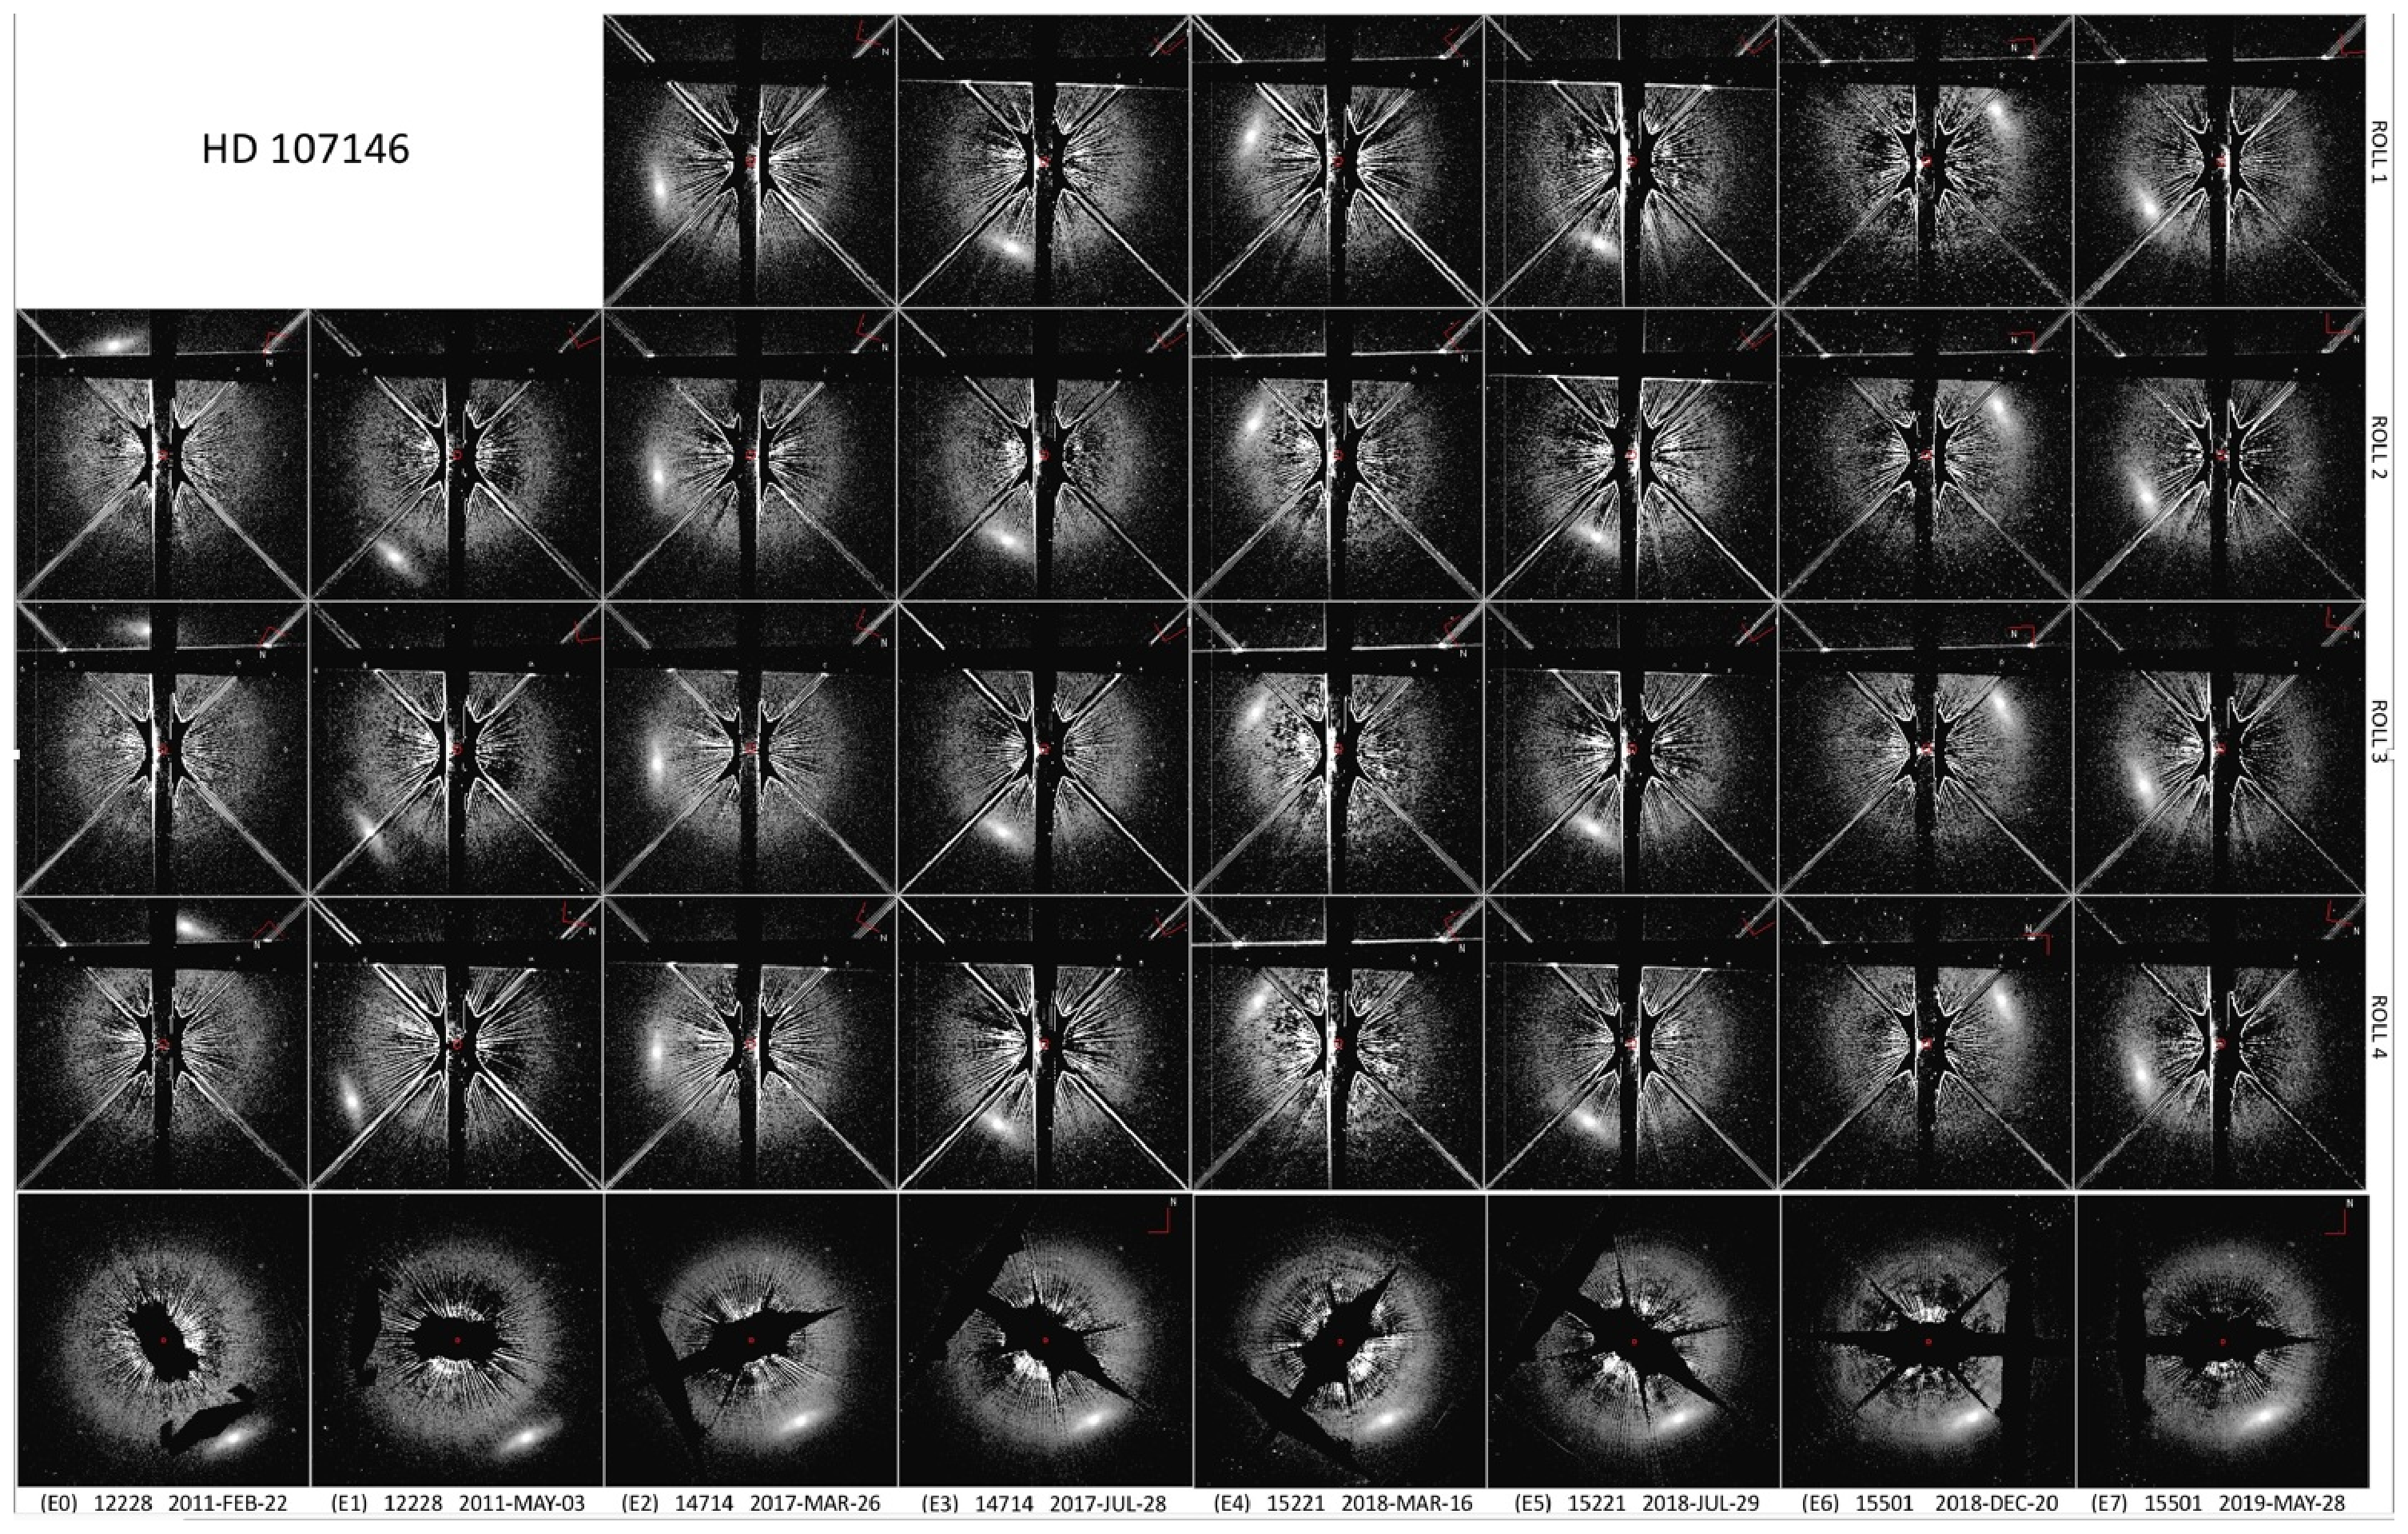
\includegraphics[width=17cm]{figures/GS01.eps}
    \caption{Top four rows (incremental differential field orientations): Visit-level reductions after step 5 (PSF template subtraction) in Science Instrument Aperture Frame with rotationally invariant PSF and disk/galaxy co-rotating with telescope orientation. Bottom row: Epoch-level reductions after step 8 (multi-roll combination in “north up” (NUP) orientation).  Central regions digitally masked as black are unsampled or degraded due to STIS occulting masks, HST diffraction spikes or other image/PSF-subtraction artifacts. Left to right columns: epoch 0 to epoch 7.}
    \label{fig:GS01}
\end{figure*}

\begin{figure*}[ht]
    \centering
    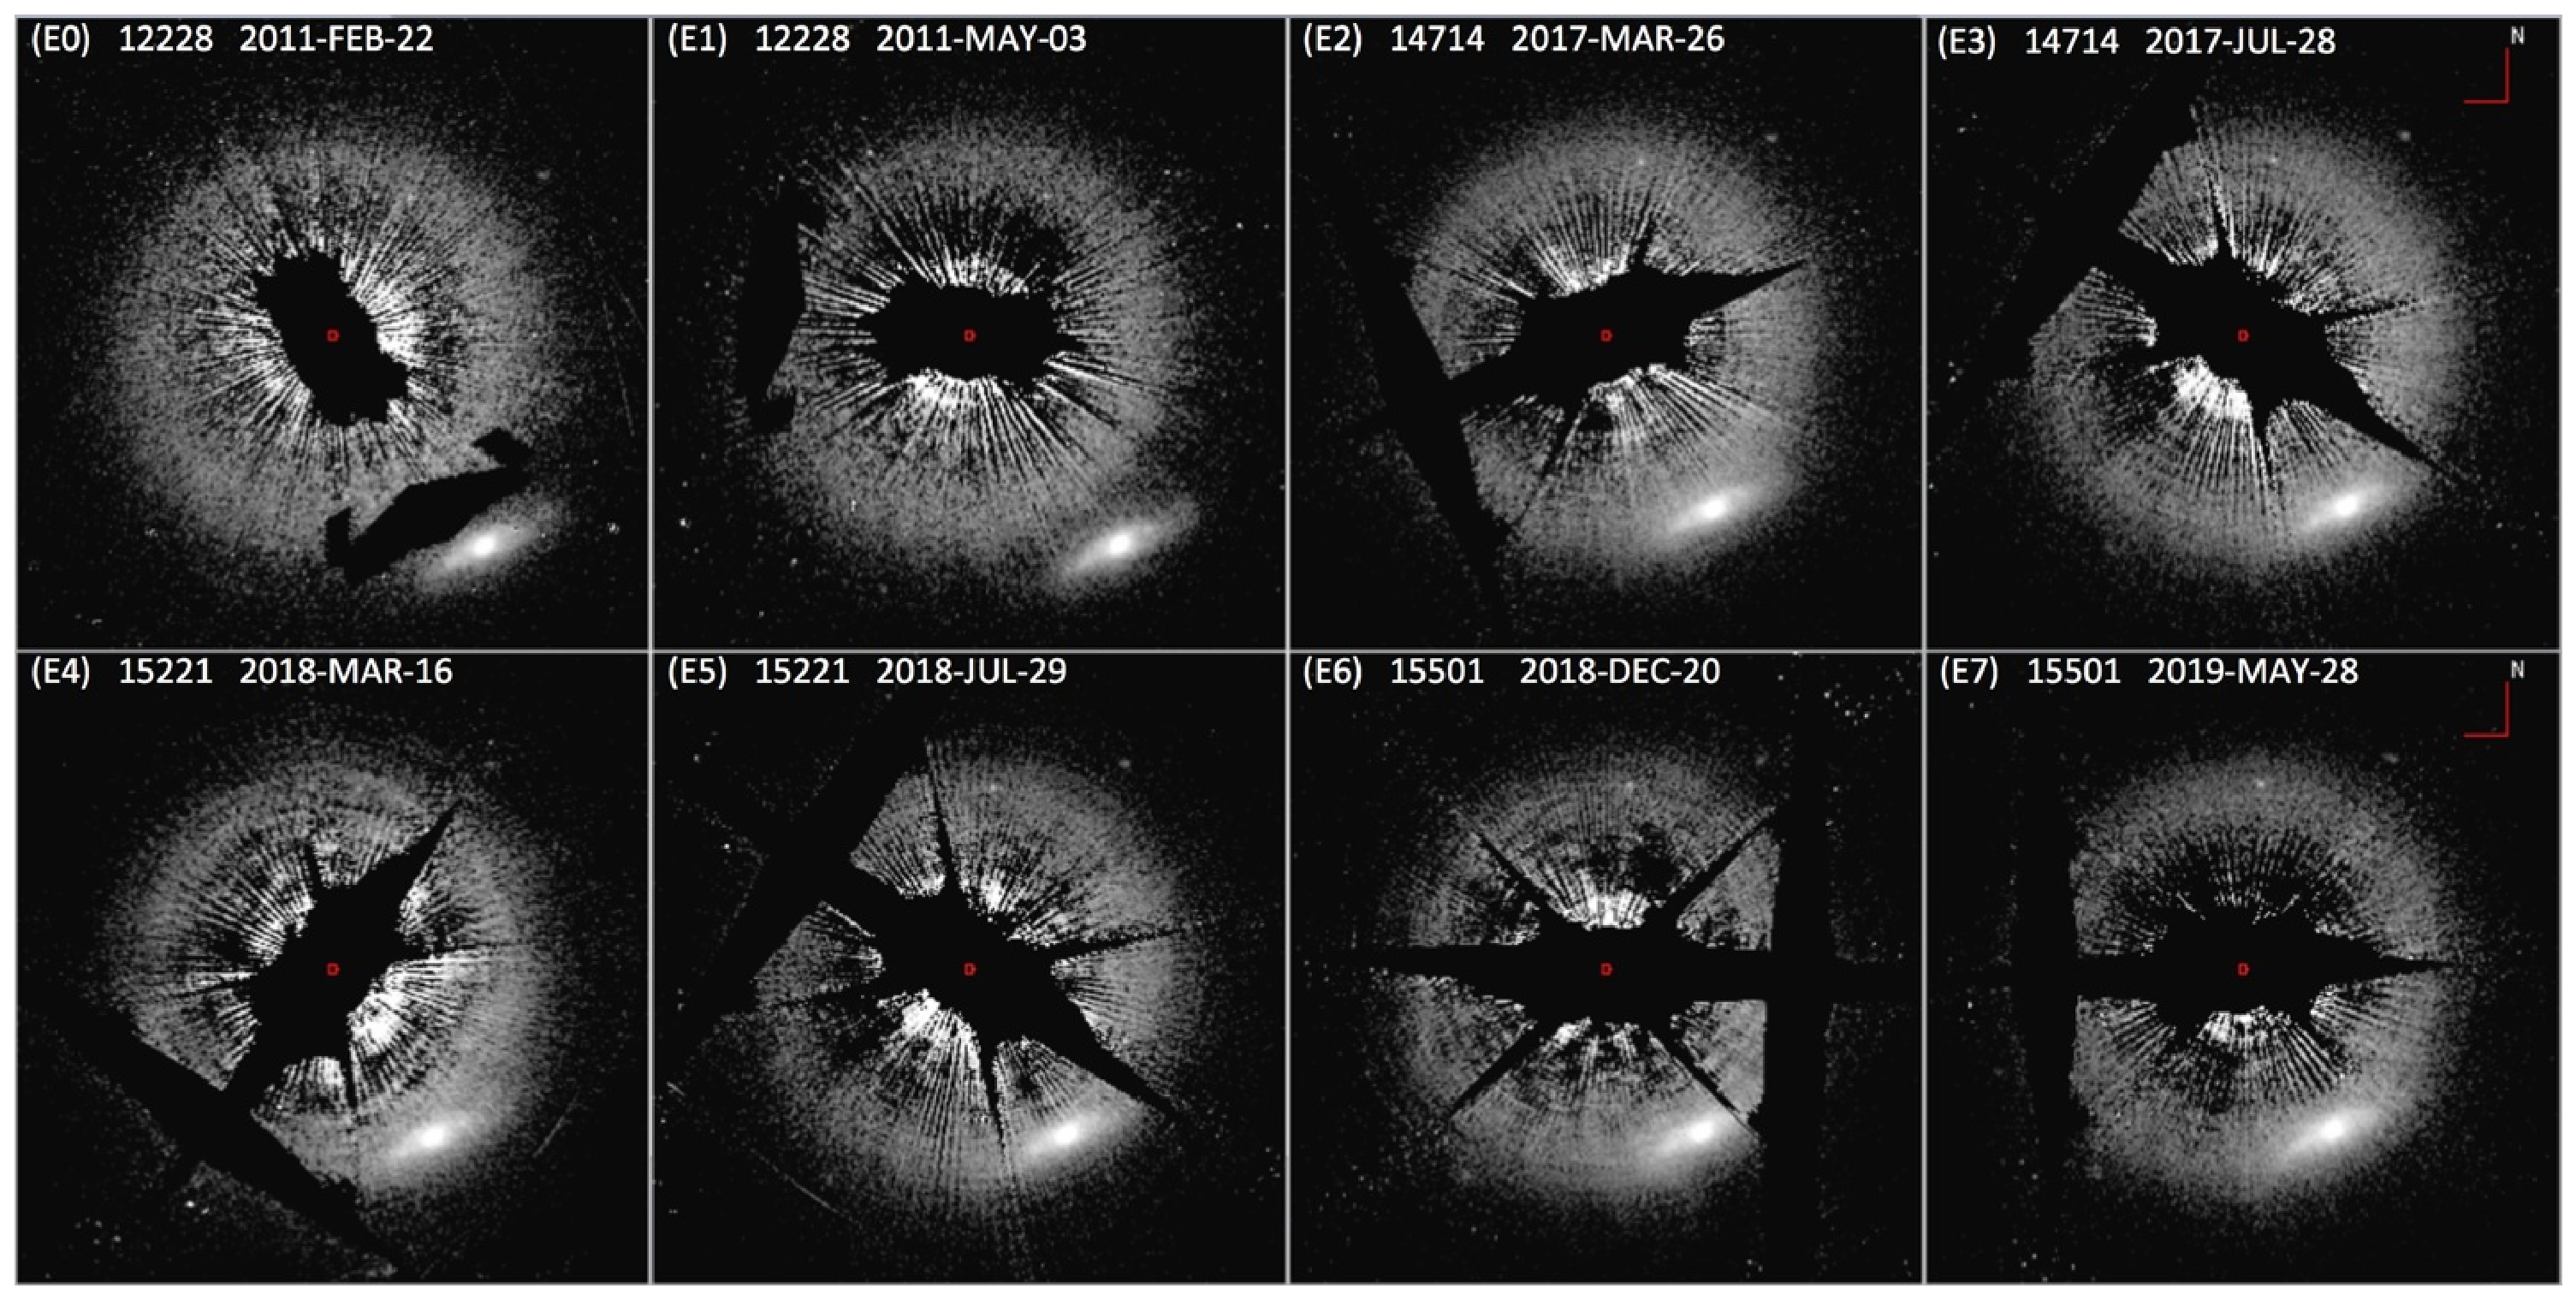
\includegraphics[width=17cm]{figures/GS02.eps}
    \caption{HD107146 debris ring transit (ingress) over background galaxy - chronologically  in panels E0 - E7. Same as \autoref{fig:GS01} bottom row (NUP) images, but illustrated in more detail.  Panels E0/E1 epochs with galaxy located at “pre-transit” periphery of debris ring re-reduced from GO 12228. Other panels (starting ~ 6 years later) are twice a year with unequal cadence per HST scheduling constraints (assuring coronagraphically obscured regions do not superimpose on the location of the galaxy with other spacecraft orientations constraints). All images are astrometrically co-registered on the obscured central star (position indicated by small red dot), are shown as log10 stretch from [-2] to [-0.7] dex counts/sec/per pixel; north up, 300x300 pixel sub-array extracts centered on target. (1 pixel = $50.077$ mas). FOVs extend further west than illustrated and provide a basis for background noise estimation.  The vermin galaxy has a peak surface brightness (Gmax) of $\sim 0.5$ counts/sec/per pixel, the disk at the same stellocentric angular distance with Dmax $\sim 0.04$ counts/sec/pixel, and a background (at large distance from the star and galaxy with RMS noise $\sigma_{rms} \approx 3\times 10^{-3}$.}
    \label{fig:GS02}
\end{figure*}



\section{Disk Scattered-light Image Modeling}
\label{sec:disk_model}

\autoref{fig:GS02} shows the circumstellar light scattered by the HD 107146 debris disk superimposed upon  the “Vermin” galaxy field at each of the eight observational epochs after stellar PSF-template subtraction removing (most of) the instrumentally diffracted and scattered starlight. To also remove the disk light from each image we apply (subtract) an observationally (not physically) informed azimuthally featureless scattered-light model of an annular disk as discussed by \cite{schneider2016extinction} (§6) to which the reader is referred for details. This surface brightness model, predicated on \cite{schneider2006discovery}\todo[inline]{Is this the right Schneider et al. 2006?}, includes a Gaussian radial taper of scattering particles at its inner and outer “edges”, azimuthal modulation with Henyey-Greenstein scattering asymmetry \citep{henyey1941diffuse}, $r^{-2}$ diminution of the stellar illumination, and is sensitive to the disk viewing geometry.

We closely follow, develop, and subtract an empirically derived best-fit disk surface brightness model in concert with the parametric prescription of \cite{schneider2016extinction}, ibid. This approach was successfully used in HST GO program 13786 to identify asymmetrical sub-structures in several other ring-like debris disks\footnote{Although, obviously, the galaxy is not intrinsic to the disk, the same disk-light rejection paradigm applies.} including HD 207129 and HD 202628. 

We illustrate with two examples. First, in \autoref{fig:GS03} left panel, to provide a fully spatially sampled image of the disk, we linearly combine the two “pre-transit” disk images closely-spaced epochs 0 and 1 from the GO 12228 data (c.f., \cite{schneider2014probing}, Figure 27) with large intra-visit roll images (see \autoref{tab:epoch_info}). Second, in \autoref{fig:GS04} illustrating disk-light rejection with (same) model subtraction with the HD 107146 debris ring superimposed upon in-transit galaxy in epoch 2 AQ image.

\begin{figure*}[ht]
    \centering
    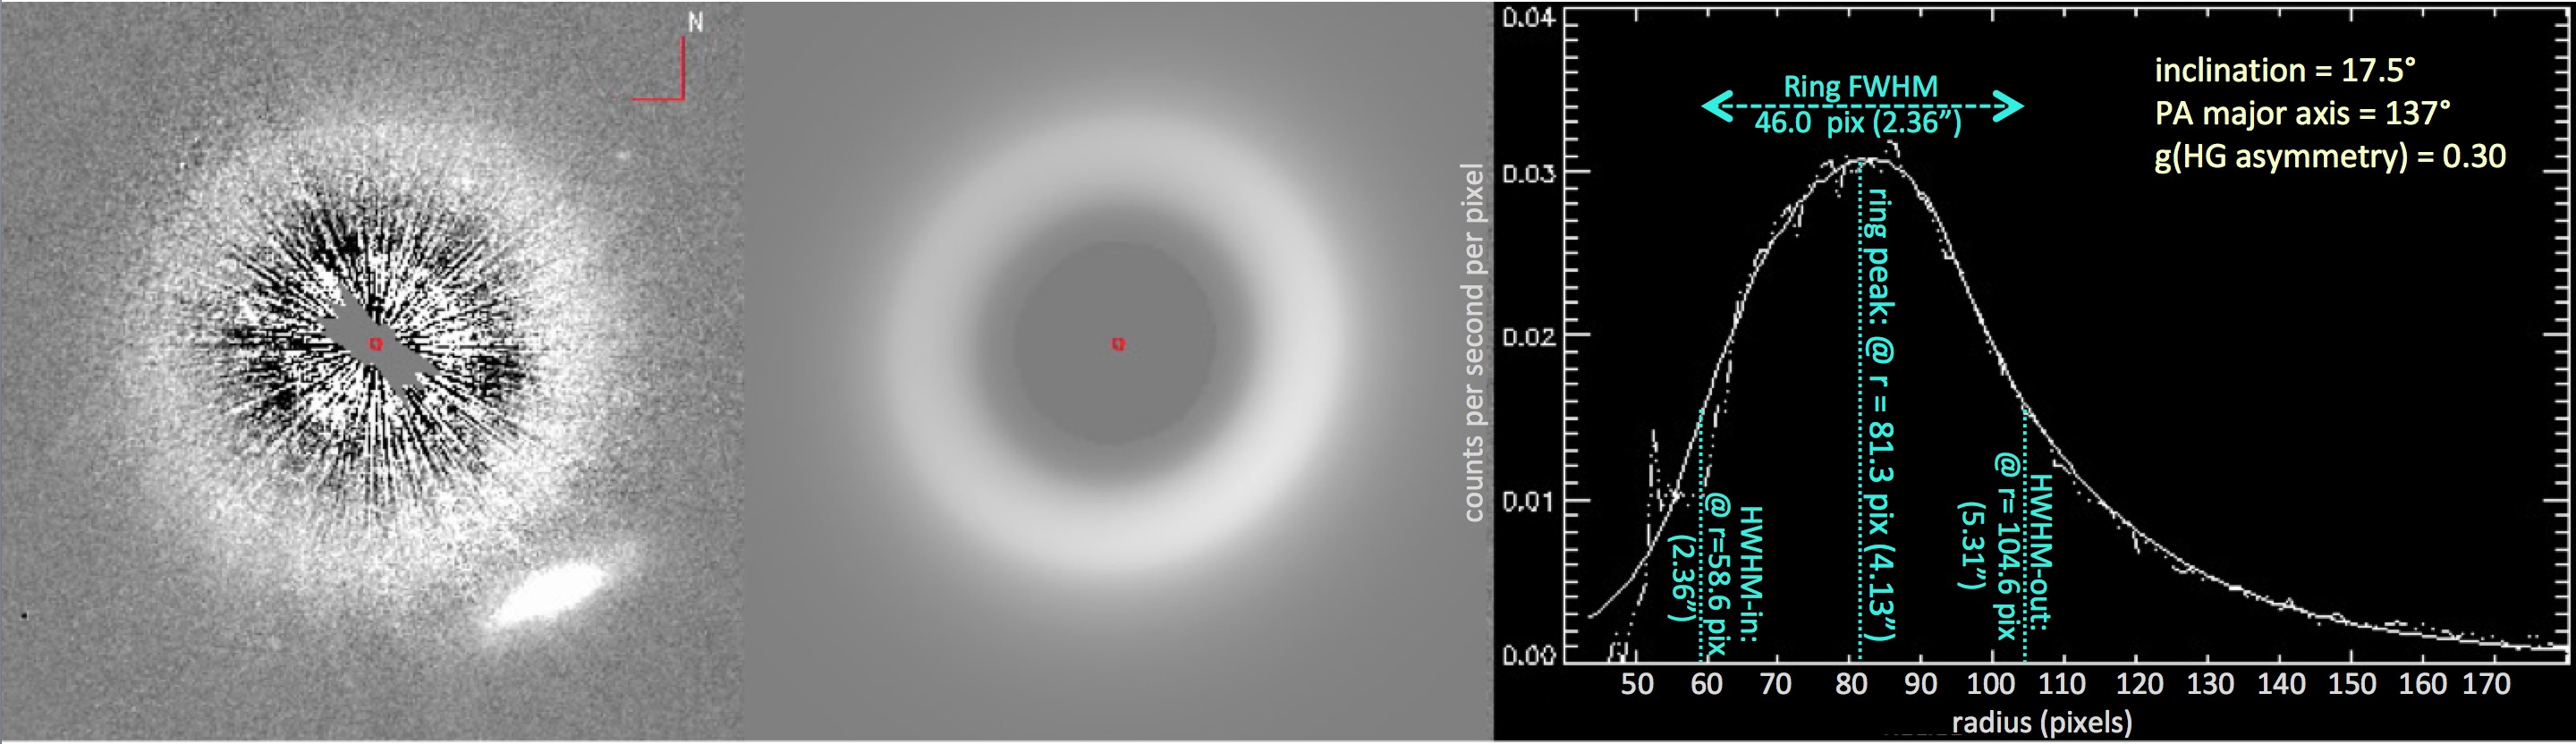
\includegraphics[width=17cm]{figures/GS03.jpg}
    \caption{Left: Epoch 0+1 AQ image of the HD 107146 debris ring fully sampled with the Vermin galaxy well separated beyond the periphery of the disk. Linear display range $\pm 0.05$ counts per second per pixel to show the structure of remaining PSF-subtraction residuals without saturating at the radius of highest surface brightness while also revealing the low level of ``pixel to pixel'' noise in the sky background at the field boundaries.  Middle: Model disk image at same display stretch derived from all eight epochs with galaxy masked. Right: Representative surface brightness radial profile/cross-section (arbitrarily along disk major axis) comparison of AQ image (solid line) vs. model comparison (dot-dashed line) showing excellent agreement at $r > 65$ pixels ($3.3''$) in region of interest of galaxy reflex motion at epochs 0 – 7 inclusive.}
    \label{fig:GS03}
\end{figure*}

\todo[inline]{Mention float32 (f4) encoding for disk model?}



% > On Mar 21, 2021, at 11:21 PM, Matthew Kenworthy <kenworthy@strw.leidenuniv.nl> wrote:
% >
% > Dear Glenn,
% >
% > I hope you and the family are keeping well in Arizona.

% And my same hopes for you in Leiden.  It has been a long year here living and working from home in sequestration. Hopefully with inoculations there will be a light at the end of this CV19 tunnel in a now shorter timescale!

% > Lukas (cc'ed) is a Leiden student working with me on the Vermin galaxy images. He's working on fitting the galaxy image in the later epoch images, so we have a couple of questions.

% Hi Lukas. It's nice to meet you at least virtually.   The HD 107146 ring transit data set is challenging but is interesting (and "fun").


% > First - is there a record of the final orientation angle of the images? We're rotating the galaxy image from the first epoch to fit to the later epochs as a free parameter, but if you have this number calculated somewhere, we can put it in as a fixed parameter.

% I am a little confused by the (perceived) need to do this.  Maybe there is a misunderstanding here?  Each of the final eight fully reduced PSF-subtracted epochal FITS images I sent by email* have already been rotated (about the location of the occulted star) to a celestial "North up" orientation. So, the orientation of the galaxy (and disk is the same (with North up) in all of the final images.

% {*In the zipped archive file: HD107146_8_EPOCHS_FULY_REDUCED.zip; filenames: HD107146_EP#_NUP_MED.fits} 


% > Second - the radial speckle residuals are overwhelming the fitting routines, so we're looking at fitting/ignoring the residuals somehow. One option would be to fit a disk model and galaxy model simultaneously to all the data and epochs. I remember you showing me an image of a model you had generated - do you have a copy of the model that we can use as part of a fitting algorithm?

% I am attaching a prior generated "best fit" scattered-light model for disk subtraction (with or without simultaneous galaxy subtraction) for all eight images.
% (Detail: In this model, the disk is not modeled interior to r = 40 pixels, but is well interior to our region of need/interest and is AOK for this need.)

% Please note when applying (subtracting from) the observed images you will need to translate (shift) the model image by (-540.45, -541.08) pixels to co-align with the observed data concentric with the star.  After that you can directly subtract.


% This, of course (simultaneous disk and galaxy) subtraction is what you really want to do.  But the disk model assumes circum-azimuthally "smooth" Henyey-Greenstein scattering. That, with other tuned parameters is a good match to the overall structure of the disk, but does not contain or alleviate the high-spatial-frequency "radial speckles" (or in STIS verbiage "spokes" that, with their residuals you say are "overwhelming" your fitting routines.  Subtracting the disk model should unbias the low-spatial frequency background, but unfortunately won't help with the spokes.  Perhaps if in some of the frames they still dominate some sort of spatial filtering might help?

% Note: When in time you develop a best (or best set) of galaxy model images, I would be very interested to see and apply those as well.

% Cheers,
% Glenn

% =============================================================================

% I wanted to add a few more explanatory words for clarity regarding image orientations, in the event Lukas is not familiar with the observing program.
% I attach a JPG graphic which helps illustrate.

% HD 107146 was first observed in optical scattered light in HST program 12228 at two epochs in 2011 spaced by several months.  At each of those epochs three images were obtained in back-to-back orbits for optical wavefront error stability, but each of those epochs spaced in time to allow for a large spacecraft roll (eelestial orientation) angle change to sample the whole disk.  When doing this in 2011 we were not concerned with the positioning of the galaxy as the goal was to fully circum-azimuthally map the disk.  So, in a few individual 2011 exposures with relatively large rolls between them, the galaxy is in some frames compromised by the HST diffraction spikes of occulting wedges.  These two sets of three images are the top three rows in columns 1 and 2  The bottom row combines the three images after rotation to common celestial North-up orientation (and median asking of the diffraction spikes that are thus eliminated).  These are the images you have.

% Starting then in 2017, about twice a year we revisited HD 107146 as the debris ring transits the background galaxy.  In these follow-ups we took 4 images per epoch taking care not to place the galaxy so not to be corrupted by the diffraction spikes or occulting wedge in any image.  The sets of 4 images at each epoch were taken with small (few  degree) 'roll dithers', i.e., at slightly different celestial orientations still within each uncorrupted aperture sector, which in subsequent image combination helps reduce the impact of the PSF subtraction high-spatial-frequency residuals.  Each of the next six columns are those 4 images at each epoch, and then in the bottom row after roll-dither masked-median combination all at he same celestial north up orientation.

% The 8 FITS files I sent earlier are the bottom row images all oriented North Up.

% FYI, the absolute calibration to the direction of celestial north is provided by the HST Pointing Control System and has an accuracy of about +/- 6 arcminutes rms in roll.  Relative roll offsets with two FGS guiding is about an order of magnitude more precise.

% Note that if you would want the pre-combined individual frames in the Science Aperture Instrument frame
% orientations (all different, not small red compass indicators) I can make those available to you.  I think you
% probably would want to work with the fully reduced images, but I am happy to provide earlier stages in processing.

% Cheers,
% Glenn


% \input{sections/01_observations}
% \input{sections/02_disk_model}
% \input{sections/03_method}
% \input{sections/04_results}
% \input{sections/05_discussion}
% \input{sections/06_conclusion}


\begin{acknowledgements}
    Acknowledgements. -- Observation campaign
\end{acknowledgements}


\bibliographystyle{aa} % style aa.bst
\bibliography{bib}


\begin{appendix}

\end{appendix}


\end{document}